\documentclass[class=article, crop=false]{standalone}
\usepackage{my_preamble}
\begin{document}
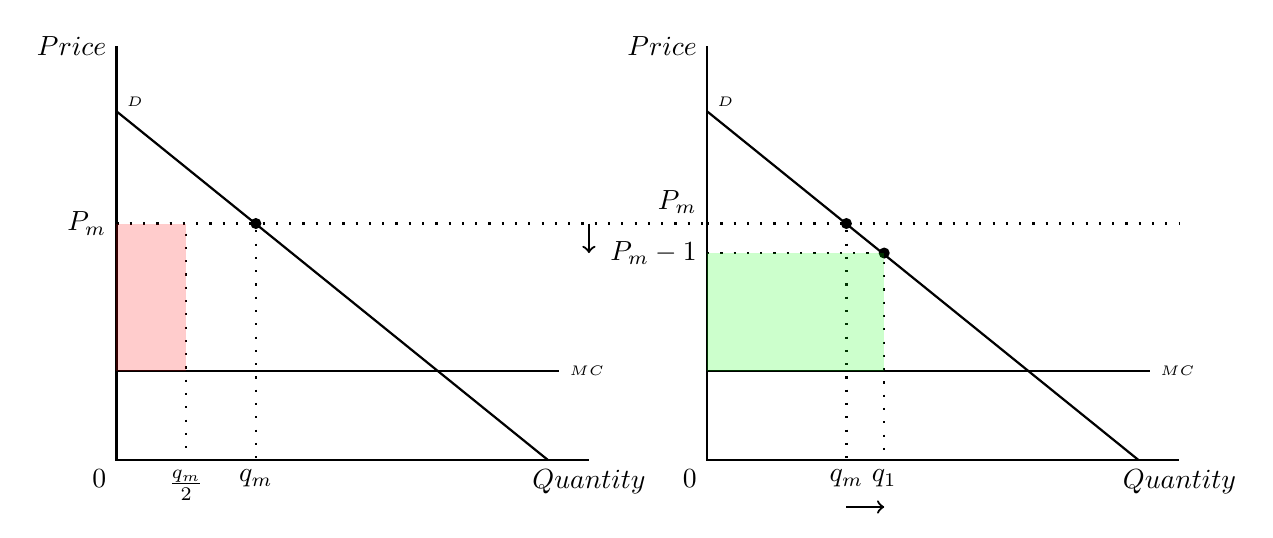
\begin{tikzpicture}[thick,font=\sffamily,scale=1.5]
	%axis
	\draw (0,3.5) node[left]{$Price$} -- (0,0) node[below left] {$0$} -- (4,0) node[below]{$Quantity$}; %graph 1
	\draw (5,3.5) node[left]{$Price$} -- (5,0) node[below left] {$0$} -- (9,0) node[below]{$Quantity$}; %graph 2
	
	%graph 1
		%curves and labels
		\draw[] (0,2.95) -- (3.65,0); %Demand
		\node[above right]at (0,2.9) {\tiny{$D$}}; %Demand label
		\draw[] (0,0.75) -- (3.75,0.75); %MC
		\node[right]at (3.75,0.75) {\tiny{$MC$}}; %MC label
		
		%nodes and dotted lines
		\draw[loosely dotted] (0,2) -- (5,2); %dotted monop price (first half)
		\draw[loosely dotted] (6.18,2) -- (9,2); %dotted monop price (second half)
		\node[style={fill=black,circle,inner sep=0pt,minimum size=4pt}] at (1.18,2) { }; %LHS node
		\draw[loosely dotted] (0,2) node[left]{$P_m$} -| node[pos=0.25,below=3mm] {}
	  (1.18,0) node[below]{$q_m$}; %Qm dotted lines
	  \draw[loosely dotted] (0,2) node[left]{} -| node[pos=0.25,below=3mm] {}
	  (0.59,0) node[below]{$\frac{q_m}{2}$}; %Qm/2 dotted lines
		
		\fill [fill=red, fill opacity=0.2] (0,2) node[left]{} -- (0.59,2) node[below left] {} -- (0.59,0.75) node[below left] {} -- (0,0.75) node[below left] {}; %fill
		
	%graph 2
		%curves and labels
		\draw[] (5,2.95) -- (8.65,0); %Demand
		\node[above right]at (5,2.9) {\tiny{$D$}}; %Demand label
		\draw[] (5,0.75) -- (8.75,0.75); %MC
		\node[right]at (8.75,0.75) {\tiny{$MC$}}; %MC label
		
		%nodes and dotted lines
		\node[style={fill=black,circle,inner sep=0pt,minimum size=4pt}] at (6.18,2) { }; %RHS node 1
		\node[style={fill=black,circle,inner sep=0pt,minimum size=4pt}] at (6.5,1.75) { }; %RHS node 2
		\draw[loosely dotted] (5,2) node[above left]{$P_m$} -| node[pos=0.25,below=3mm] {}
	  (6.18,0) node[below]{$q_m$}; %Qm dotted lines
	  \draw[loosely dotted] (5,1.75) node[left]{$P_m-1$} -| node[pos=0.25,below=3mm] {}
	  (6.5,0) node[below]{$q_1$}; %Pm-1 dotted lines
	  
		%arrows
		\draw [->] (6.18,-0.4) -- (6.5,-0.4); %x arrow
		\draw [->] (4,2) -- (4,1.75); %y arrow
  
	\fill [fill=green, fill opacity=0.2] (5,1.75) node[left]{} -- (6.5,1.75) node[below left] {} -- (6.5,0.75) node[below left] {} -- (5,0.75) node[below left] {}; %fill
  
\end{tikzpicture}
%\node[above right]at (1.8,1.5) {\tiny{$SRAS_{0}$}};
\end{document}